% Options for packages loaded elsewhere
\PassOptionsToPackage{unicode}{hyperref}
\PassOptionsToPackage{hyphens}{url}
%
\documentclass[
]{article}
\usepackage{lmodern}
\usepackage{amssymb,amsmath}
\usepackage{ifxetex,ifluatex}
\ifnum 0\ifxetex 1\fi\ifluatex 1\fi=0 % if pdftex
  \usepackage[T1]{fontenc}
  \usepackage[utf8]{inputenc}
  \usepackage{textcomp} % provide euro and other symbols
\else % if luatex or xetex
  \usepackage{unicode-math}
  \defaultfontfeatures{Scale=MatchLowercase}
  \defaultfontfeatures[\rmfamily]{Ligatures=TeX,Scale=1}
\fi
% Use upquote if available, for straight quotes in verbatim environments
\IfFileExists{upquote.sty}{\usepackage{upquote}}{}
\IfFileExists{microtype.sty}{% use microtype if available
  \usepackage[]{microtype}
  \UseMicrotypeSet[protrusion]{basicmath} % disable protrusion for tt fonts
}{}
\makeatletter
\@ifundefined{KOMAClassName}{% if non-KOMA class
  \IfFileExists{parskip.sty}{%
    \usepackage{parskip}
  }{% else
    \setlength{\parindent}{0pt}
    \setlength{\parskip}{6pt plus 2pt minus 1pt}}
}{% if KOMA class
  \KOMAoptions{parskip=half}}
\makeatother
\usepackage{xcolor}
\IfFileExists{xurl.sty}{\usepackage{xurl}}{} % add URL line breaks if available
\IfFileExists{bookmark.sty}{\usepackage{bookmark}}{\usepackage{hyperref}}
\hypersetup{
  hidelinks,
  pdfcreator={LaTeX via pandoc}}
\urlstyle{same} % disable monospaced font for URLs
\usepackage{graphicx,grffile}
\makeatletter
\def\maxwidth{\ifdim\Gin@nat@width>\linewidth\linewidth\else\Gin@nat@width\fi}
\def\maxheight{\ifdim\Gin@nat@height>\textheight\textheight\else\Gin@nat@height\fi}
\makeatother
% Scale images if necessary, so that they will not overflow the page
% margins by default, and it is still possible to overwrite the defaults
% using explicit options in \includegraphics[width, height, ...]{}
\setkeys{Gin}{width=\maxwidth,height=\maxheight,keepaspectratio}
% Set default figure placement to htbp
\makeatletter
\def\fps@figure{htbp}
\makeatother
\setlength{\emergencystretch}{3em} % prevent overfull lines
\providecommand{\tightlist}{%
  \setlength{\itemsep}{0pt}\setlength{\parskip}{0pt}}

\date{}

\begin{document}

\hypertarget{design-documentation}{%
\section{Design Documentation}\label{design-documentation}}

\hypertarget{overview}{%
\subsection{Overview}\label{overview}}

\begin{figure}
\centering
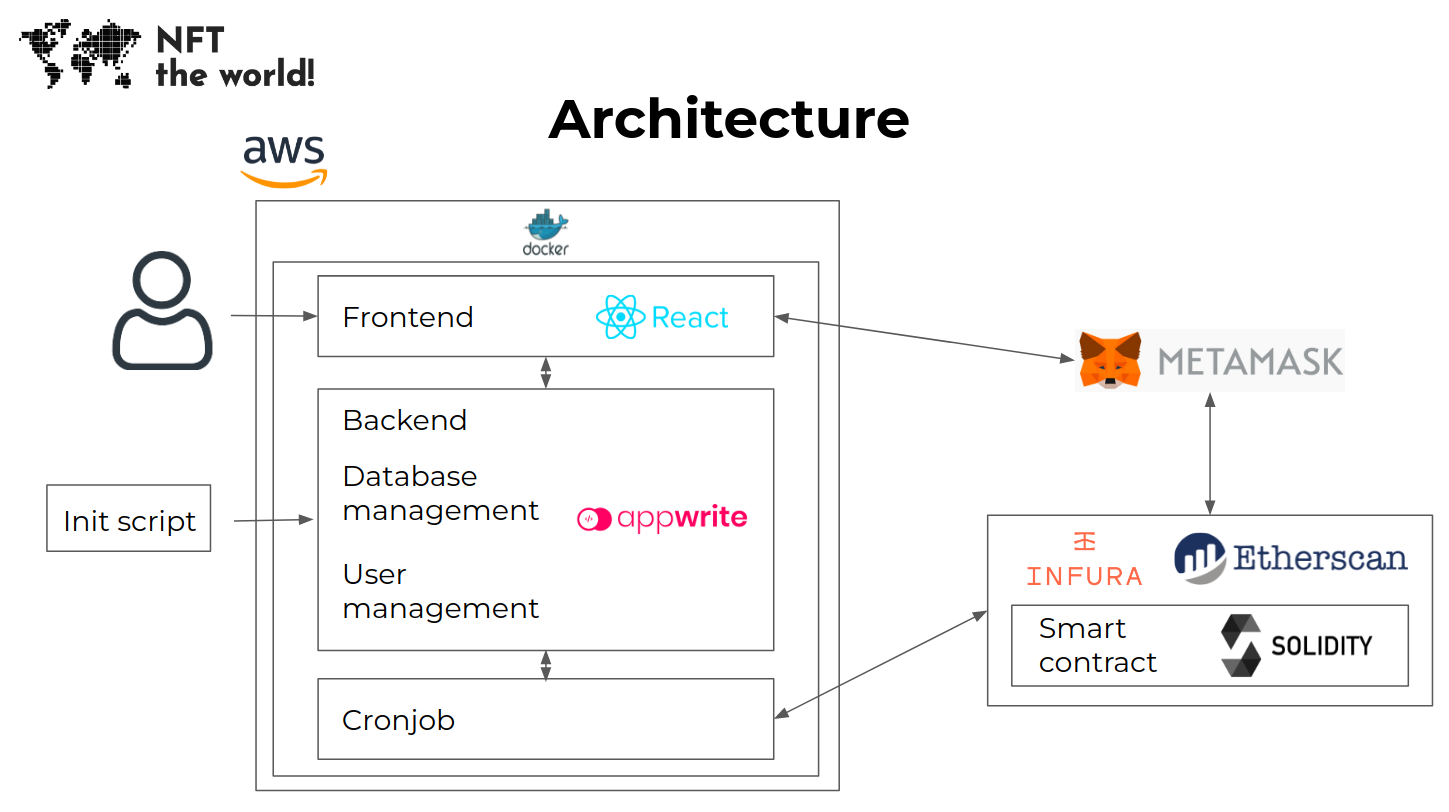
\includegraphics{images/architecture.png}
\caption{Architecture}
\end{figure}

For more details, there are \texttt{README.md} files within some
directories like \texttt{./frontend/} and \texttt{./blockchain/}.

There is also a wiki page which gives an overview over the repository
artifacts.

You'll find a link in the Software architecture description is
mentioned.

\hypertarget{decentralization}{%
\subsection{Decentralization}\label{decentralization}}

To ensure, that the sold NFTs don't depend on our server deployment, we
aimed for a design that allows users to fully utilize their tokens
(whatever that means) even without our backend server. In order to
achieve that, images of NFTs are stored in the
\href{https://en.wikipedia.org/wiki/InterPlanetary_File_System}{InterPlanetary
File System}. The Token themselves are store in the
\href{https://en.wikipedia.org/wiki/Ethereum}{Ethereum Blockchain}. (In
the standard configuration the
\href{https://eth.wiki/fundamentals/testnets}{Kovan Testnet} it used
which involves no real money.)

\hypertarget{scalability}{%
\subsection{Scalability}\label{scalability}}

Although all the important functionality is decentralized and highly
resilient, our service is built on docker containers and thus easily
scalable, to ensure smooth operations during times with high traffic
(drops).

\hypertarget{security}{%
\subsection{Security}\label{security}}

All important transactions happen directly on the blockchain, meaning
that the ownership of the NFTs is tracked outside the webservice. The
only user data, that is stored in our backend are:

\begin{itemize}
\tightlist
\item
  mail addresses
\item
  usernames
\item
  passwords (salted and hashed)
\item
  group memberships (Partner, Admin)
\item
  announcements (some kind of news messages shown in the app)
\end{itemize}

Appwrite implements some default level of security when using API-calls
like a minimum password, one-time password recovery, limited number of
sequential requests (to prevent spam), session keys and privileges.

\end{document}
